% cover-lulu-quarto.tex

% make a cover PDF for lulu.com's Crown Quarto booksize.

% note: Lulu will flatten this PDF and get the colors wrong. Convert
% this PDF to PNG first (eg, using GIMP: just import at 300dpi then
% export as PNG).

\documentclass{memoir}
\usepackage[sfdefault]{universalis}
\usepackage[osf]{Baskervaldx} % oldstyle figures

\newcommand{\olpath}{../../}

\usepackage[absolute,overlay]{textpos}
\usepackage{rotating}
\usepackage{xcolor}

\definecolor{leadbeater}{RGB}{248,154,14}

% lulu.com's instructions:
% Spine width: 59.351 Postscript points wide (2.094 cm) (247 px)
% Spine begins 545 Postscript points (19.224 cm) (2271 px) from the left.
% Total cover width: 1149.351 X 715 Postscript points (40.541 cm X 25.220 cm) (4789px X 2979px)

\newlength{\coverheight}
\newlength{\coverwidth}
\newlength{\spinewidth}
\newlength{\spinepos} % spine starts here, width = \spinewidth
\newlength{\coverpos} % front cover starts here, width = \spinepos

\setlength{\coverheight}{715bp}
\setlength{\coverwidth}{1149.351bp}
\setlength{\spinewidth}{59.351bp}
\setlength{\spinepos}{545bp}

% \coverpos = \spinepso + \spinewidth
\setlength{\coverpos}{\spinepos}
\addtolength{\coverpos}{\spinewidth}

% set stock size to total width & height of cover 
\setstocksize{\coverheight}{\coverwidth}

% pagesize = stocksize
\settrimmedsize{\stockheight}{\stockwidth}{*}
\settrims{0pt}{0pt}

% no margins or headers
\setlrmarginsandblock{0pt}{0pt}{*}
\setheadfoot{0pt}{0pt}
\setulmarginsandblock{0pt}{0pt}{*}
\setheadfoot{0pt}{0pt}
\setlength{\headsep}{0pt}


% finalize the page layout
\checkandfixthelayout[fixed]
\typeoutlayout

\color{black}

\begin{document}
% no folios
\pagestyle{empty}

% set back background to Matt's orange

\pagecolor{leadbeater}

% make a spine
\begin{textblock*}{\spinewidth}(\spinepos,0bp)%
\noindent\hfil\rotatebox{-90}{% make spine text readable when book is lying cover up
      \hbox to \coverheight{\hfil
          \huge\sffamily\bfseries\color{black}
            Sets, Logic, Computation\hfil F17\hspace{1cm}}}\hfil
\end{textblock*}
\newbox\adjust
% make front cover
\begin{textblock*}{\spinepos}(\coverpos,0pt)
  \noindent\hfil
  \begin{minipage}[b][\coverheight][s]{.8\spinepos}
    \vspace{2cm}
    \begin{raggedright}
      \fontsize{32pt}{34pt}\selectfont\bfseries\sffamily%
      Sets, Logic, Computation\\
      \normalfont\fontsize{18pt}{0pt}\selectfont\bfseries\itshape%
      \rule{.8\spinepos}{5pt}\\[5pt]
      An Open Logic Text
    \end{raggedright}
    \noindent\vskip2cm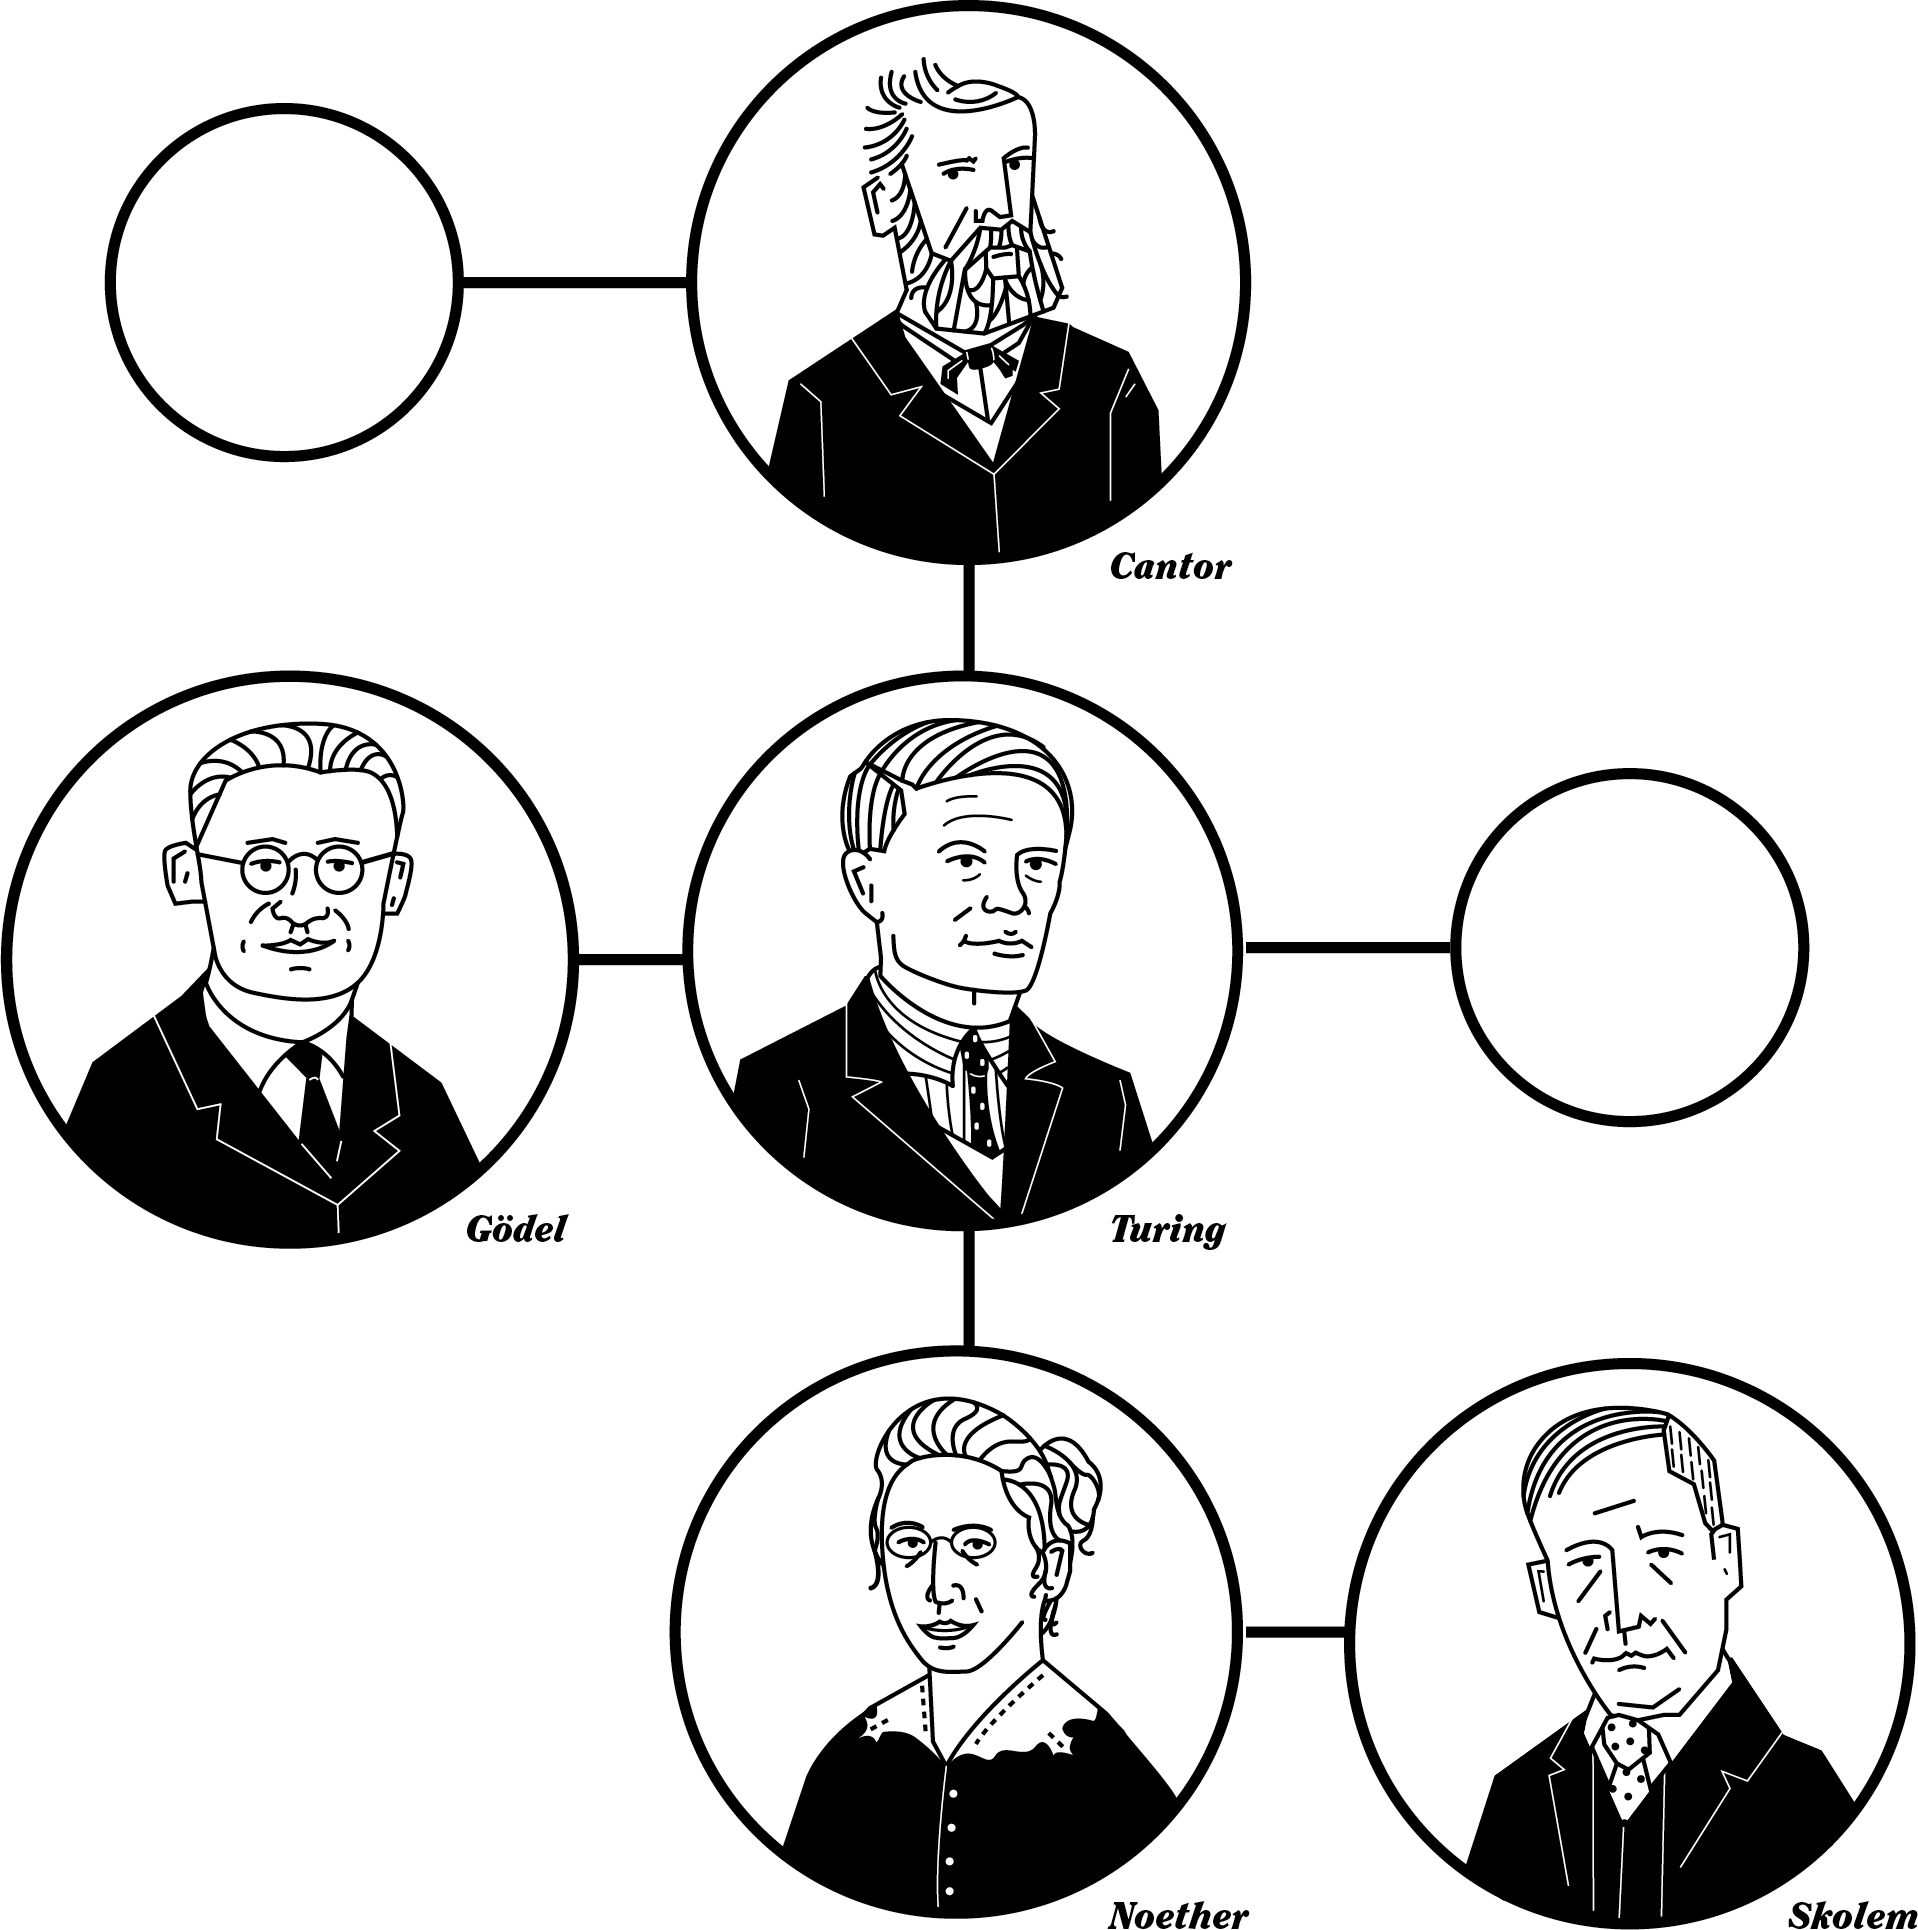
\includegraphics[width=.8\spinepos]{illustrations/Cover}
    \par\noindent
    \vskip 1.5cm
    \includegraphics[width=1cm]{assets/cc.pdf}
    \includegraphics[width=1cm]{assets/by.pdf}
    \includegraphics[width=1cm]{assets/remix.pdf}
    \normalfont\fontsize{16pt}{0pt}\selectfont\bfseries\sffamily%
    \hfill Fall 2017 \textit{bis}
  \end{minipage}
  \hfil
  \end{textblock*}

% make back cover
\begin{textblock*}{\spinepos}(0pt,0pt)
  \noindent\hfil
  \begin{minipage}[b][\coverheight][b]{.8\spinepos}
\begin{minipage}[b]{.9cm}
\includegraphics[width=.9cm]{\olpath/assets/logos/by}
\includegraphics[width=.9cm]{\olpath/assets/logos/cc}
\includegraphics[width=.9cm]{\olpath/assets/logos/remix}
\end{minipage}
\hspace{.3cm}
\begin{minipage}[b]{5cm}
\fontsize{8.5pt}{1em}\selectfont\textit{Sets, Logic, Computation}
by Richard Zach is licensed under a Creative Commons Attribution 4.0
International License. It is based on \textit{The Open Logic Text} by
the Open Logic Project (openlogicproject.org), used under a Creative
Commons Attribution 4.0 International License.
\end{minipage}
\hfill\color{black}
%\colorbox{white}{\includegraphics[width=1.75in]{isbn_barcode}}
\includegraphics[width=2.7cm]{\olpath/assets/logos/openlogic-logo-bw}
\vspace*{1cm}
  \end{minipage}
  \hfil
  \end{textblock*}

\end{document}
